\subsection{Transport by many molecular motors}
\subsubsection{The symmetric exclusion process (SEP)}
\begin{figure}[H]
	\centering
	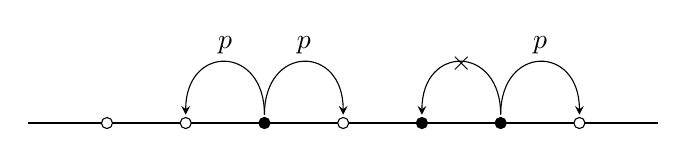
\begin{tikzpicture}[>=stealth]
		\draw (0,0)--(8,0);
		\foreach \x \y in {1/white,2/white,3/black,4/white,5/black,6/black,7/white}{
			\draw[fill=\y] (\x,0)circle(2pt);
		}
		\def\k{1}
		\draw[->,shorten <= 3pt, shorten >= 3pt] (3,0) .. controls +(0,\k) and +(0,\k) .. (2,0)node[midway,above]{$p$};
		\draw[->,shorten <= 3pt, shorten >= 3pt] (3,0) .. controls +(0,\k) and +(0,\k) .. (4,0)node[midway,above]{$p$};
		\draw[->,shorten <= 3pt, shorten >= 3pt] (6,0) .. controls +(0,\k) and +(0,\k) .. (5,0)node[midway]{$\times$};
		\draw[->,shorten <= 3pt, shorten >= 3pt] (6,0) .. controls +(0,\k) and +(0,\k) .. (7,0)node[midway,above]{$p$};
	\end{tikzpicture}
\end{figure}
\textbf{\underline{\smash{Evolution of the density at a given site $n$}}}:\vspace{3mm}\\
Let $P_{n,m}(t)$ be the joint probability that sites $n,m$ are occupied, $P_{n,\bar{m}}$ the probability that $n$ is occupied but $m$ isn't and similar.\\
For the SEP the single-particle density evovles as:
\begin{equation*}
	\frac{dP_n}{dt}=\sum\limits_m\left(P_{\bar{n},m}-P_{n,\bar{m}}\right)
\end{equation*}
where the hopping rate $p=1$. The sum runs over all neiboring sites of $n$. The joint probabilities fulfill the relation
\begin{equation*}
	P_{n,m}(t)+P_{n,\bar{m}}(t)=P_n(t) \quad \& \quad P_{n,m}(t) + P_{\bar{n},m}(t)=P_m
\end{equation*}
\begin{equation*}
	\frac{dP_n}{dt}=\sum\limits_n\left(P_m-P_n\right)
\end{equation*}
$\to$ The evolution of the density is the same as for symmetric diffusion of a single particle, irrespective of the particle density.\\
The differences to single particle diffusion show up for the dynamics of a given tracer particle. There the typical displacement grows as:
\begin{equation*}
	\sqrt{\left\langle x^2\right\rangle}=At^\frac{1}{4} \text{ with } A=\left(\frac{2}{\sqrt{\pi}}\frac{1-c}{c}\right)^\frac{1}{2}
\end{equation*}
\subsubsection{The Asymmetric Exclusion Process (ASEP)}
The ASEP is a stochastic process that combines exclusion, stochasticity and directionality, and thereby the essential characteristics of the motor dynamics, except their finite runlength.\\
A particle hops to the right with rate $p$ and to the left with rate $q$
\begin{figure}[H]
	\centering
	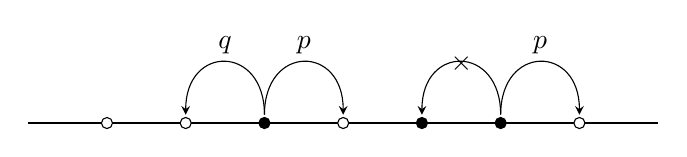
\begin{tikzpicture}[>=stealth]
		\draw (0,0)--(8,0);
		\foreach \x \y in {1/white,2/white,3/black,4/white,5/black,6/black,7/white}{
			\draw[fill=\y] (\x,0)circle(2pt);
		}
		\def\k{1}
		\draw[->,shorten <= 3pt, shorten >= 3pt] (3,0) .. controls +(0,\k) and +(0,\k) .. (2,0)node[midway,above]{$q$};
		\draw[->,shorten <= 3pt, shorten >= 3pt] (3,0) .. controls +(0,\k) and +(0,\k) .. (4,0)node[midway,above]{$p$};
		\draw[->,shorten <= 3pt, shorten >= 3pt] (6,0) .. controls +(0,\k) and +(0,\k) .. (5,0)node[midway]{$\times$};
		\draw[->,shorten <= 3pt, shorten >= 3pt] (6,0) .. controls +(0,\k) and +(0,\k) .. (7,0)node[midway,above]{$p$};
	\end{tikzpicture}
\end{figure}
\noindent We consider $p>q$ and, for convenience, $p+q=1$. The main qualitative features are observed for any strength of the relative bias. Therefore, often $p=1$ (TASED for Totally Asymmetric Exclusion Process) is chosen.\vspace{3mm}\\
\textbf{\underline{\smash{Steady states}}}\vspace{2mm}\\
A state of the ASEP is specified by the location of all particles. There is a configuration $\mathcal{C}$. The probability $P(\mathcal{C},t)$ to find a configuration $\mathcal{C}$ at time $t$ evolves according to:
\begin{equation*}
	\frac{dP(\mathcal{C},t)}{dt}=\sum\limits_{\mathcal{C}'}\big(P(\mathcal{C}',t)W(\mathcal{C}'\to\mathcal{C})\big)-P(\mathcal{C},t)\sum\limits_{\mathcal{C}'}W(\mathcal{C}\to\mathcal{C}')
\end{equation*}
In a steady state one obviously gets:
\begin{equation*}
	\sum\limits_{\mathcal{C}'}P_S(\mathcal{C}')W(\mathcal{C}'\to\mathcal{C})=P(\mathcal{C})\sum\limits_{\mathcal{C}'}W(\mathcal{C}\to\mathcal{C}')
\end{equation*}
For an equilibrium system the stationary solution is given by
\begin{equation*}
	P_S(\mathcal{C})=P_{eq}(\mathcal{C})=\frac{1}{Z}e^{-\beta E(\mathcal{C})}
\end{equation*}
This is not true for non-equilibrium processes, where the stationary master equation has to be solved. For non-equilibrium system the detailed balance condition does not hold in general.\vspace{2mm}\\
\textbf{\underline{\smash{Steady states on a ring}}}\vspace{3mm}\\
The steady state on a ring can be obtained by arranging particles into "{}islands".
\begin{figure}[H]
	\centering
	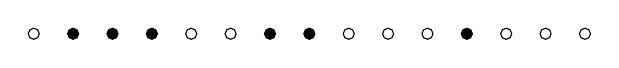
\begin{tikzpicture}
		\foreach \x \y in {1/white,2/black,3/black,4/black,5/white,6/white,7/black,8/black,9/white,10/white,11/white,12/black,13/white,14/white,15/white}{
			\draw[fill=\y] ({0.5*\x-0.5},0)circle(2pt)coordinate(C\x);
		}
	\end{tikzpicture}
\end{figure}
\noindent Here, we have $N=15$, $I(\mathcal{C})=3$ and $M=6$.\\
Now in a given time interval $dt$ the probability of learning $\mathcal{C}$ is given by $I(\mathcal{C})P_S(\mathcal{C})dt$, since only the rightmost particle of an island my hop.
